%Version 3 October 2023
%%%%%%%%%%%%%%%%%%%%%%%%%%%%%%%%%%%%%%%%%%%%%%%%%%%%%%%%%%%%%%%%%%%%%%
%% scMetaIntel-Hub article — Springer Nature (sn-nature) format
%% Submit as one .tex document; figures attached separately.
%%%%%%%%%%%%%%%%%%%%%%%%%%%%%%%%%%%%%%%%%%%%%%%%%%%%%%%%%%%%%%%%%%%%%%

\documentclass[sn-nature]{sn-jnl}

\usepackage{graphicx}
\graphicspath{{../article_figures/}}
\usepackage{multirow}
\usepackage{amsmath,amssymb,amsfonts}
\usepackage{booktabs}
\usepackage{xcolor}
\usepackage{textcomp}
\usepackage{url}
\usepackage{subcaption}
\usepackage{enumitem}

\raggedbottom

\begin{document}

\title[scMetaIntel-Hub]{scMetaIntel-Hub: Benchmarking Local Large Language Models for Privacy-Preserving Single-Cell Dataset Discovery}

\author*[1]{\fnm{Zeyu} \sur{Fu}}\email{zeyu.fu@example.edu}

\affil*[1]{\orgdiv{Department of Bioinformatics},
  \orgname{University},
  \orgaddress{\city{City}, \state{State}, \country{Country}}}

\abstract{The Gene Expression Omnibus (GEO) accumulates over 2{,}000 single-cell
genomics datasets per year, yet discovery remains confined to keyword search
with no semantic reasoning or metadata-aware retrieval. Cloud-hosted large
language models (LLMs) can parse complex queries and generate cited answers,
but their use raises data-governance concerns for institutions handling
restricted or unpublished metadata. We present scMetaIntel-Hub, a fully local
pipeline that converts natural-language queries into grounded, cited answers
over single-cell metadata. The system requires no cloud API access and
operates exclusively on GEO metadata and PubMed abstracts. We benchmark 51
local LLMs from 16 architectural families (66 configurations including
chain-of-thought ablation) across eight domain-specific tasks on a curated
corpus of 2{,}189 GEO studies and 171 evaluation queries. A 32B model (aya-expanse-32b, composite 0.779) and a 4B model
(qwen3.5-4b, composite 0.779) are statistically tied at first rank, both
outperforming 14B alternatives. Hybrid retrieval with organism filtering
matches or exceeds neural reranking at half the latency. Quantisation from
8-bit to 4-bit incurs negligible quality loss with 1.4x throughput gain. The corpus, queries, and all benchmark
code are publicly available.}

\keywords{single-cell genomics, large language models, metadata
  intelligence, benchmark, retrieval-augmented generation,
  local inference}

\maketitle

%% ====================================================================
\section{Introduction}\label{sec:intro}
%% ====================================================================

Single-cell genomics has reshaped the study of cellular heterogeneity in
development, disease, and tissue homeostasis. The Gene Expression Omnibus
(GEO) now hosts more than 15{,}000 single-cell datasets spanning over 40
organisms, with roughly 2{,}000 new series deposited each
year~\cite{barrett2013ncbi}. Complementary repositories such as CZ
CELLxGENE~\cite{megill2021cellxgene} and the Human Cell
Atlas~\cite{regev2017human} further expand the landscape. This growth
makes manual curation and keyword-based search increasingly inadequate for
dataset discovery.

GEO DataSets provides Boolean queries over titles and summaries; CELLxGENE
offers faceted filtering by organism, tissue, and disease. Neither supports
semantic queries such as ``\textit{Find scRNA-seq datasets studying the
tumour microenvironment in colorectal cancer},'' nor can they synthesise
cross-study answers grounded in specific accessions. Researchers must
instead scan result lists, read abstracts, and manually compile findings---a
workflow that scales poorly.

Large language models (LLMs) address this gap through natural-language
understanding, structured metadata extraction, ontology normalisation, and
retrieval-augmented generation (RAG)~\cite{lewis2020retrieval}. Cloud-hosted
models such as GPT-4~\cite{openai2023gpt4} achieve strong performance on
biomedical QA benchmarks~\cite{nori2023capabilities}, but their use conflicts
with institutional policies on data governance when queries involve
restricted, unpublished, or pre-publication metadata. Locally deployed
open-weight models eliminate this concern, yet no systematic evaluation
exists for the expanding ecosystem of local LLMs (Qwen, Llama, Gemma,
Mistral, Phi, and others) on the specific tasks required for single-cell
metadata intelligence.

Existing LLM benchmarks target general knowledge (MMLU~\cite{hendrycks2021measuring}),
mathematical reasoning (GSM8K~\cite{cobbe2021training}), or broad biomedical
QA (PubMedQA~\cite{jin2019pubmedqa}, MedQA~\cite{jin2021disease}). None
evaluate structured query parsing from natural language, metadata extraction
from GEO abstracts, ontology normalisation against Cell Ontology
(CL)~\cite{diehl2016cell}, Uberon~\cite{mungall2012uberon}, and Mondo, or
grounded answer generation with accession-level citations. These are distinct
tasks from literature question answering and require dedicated benchmarks.

We present scMetaIntel-Hub with four contributions:

\begin{enumerate}[leftmargin=2em, itemsep=2pt]
  \item A \textbf{metadata-only intelligence pipeline} (parse $\to$ embed
    $\to$ retrieve $\to$ assemble $\to$ answer) that operates exclusively
    on GEO metadata and PubMed abstracts, without expression matrices or
    cloud dependencies.

  \item A \textbf{systematic local LLM benchmark} evaluating 51 models from
    16 families in 66 configurations (including chain-of-thought ablation)
    across eight domain-specific tasks, using a curated corpus of 2{,}189
    enriched GEO studies and 171 evaluation queries.

  \item An \textbf{empirically validated pipeline recipe}: hybrid retrieval
    with organism filtering outperforms neural reranking; a 4B model
    statistically ties the top 32B model; 4-bit quantisation incurs
    negligible quality loss.

  \item A \textbf{curated evaluation resource}: 2{,}189 enriched GSE
    metadata files, 171 queries across seven categories and three difficulty
    levels, and fully reproducible benchmark scripts.
\end{enumerate}

%% ====================================================================
\section{Methods}\label{sec:methods}
%% ====================================================================

\subsection{Data collection and curation}\label{sec:data}

We assembled a corpus of 2{,}189 GEO Series (GSE) accessions representing
single-cell experiments. For each accession, structured metadata was
retrieved from the GEO SOFT format (title, summary, overall design,
organism, platform, sample characteristics) and linked PubMed abstracts were
obtained via NCBI E-utilities. A multi-stage cleaning pipeline processed the
raw metadata: (i)~text-presence filtering to retain annotations recoverable
from the study abstract; (ii)~cell-line removal from tissue lists;
(iii)~disease term migration from tissue to disease fields; (iv)~removal of
non-disease terms (``control,'' ``normal''); (v)~text-based gap filling for
studies with missing disease or cell-type annotations.

The resulting corpus spans 42 organisms (50.8\% \textit{Homo sapiens},
38.9\% \textit{Mus musculus}), with tissue annotations for 83.8\% of
studies, disease annotations for 44.8\%, cell-type annotations for 72.6\%,
PubMed linkage for 69.0\%, and complete document text for all 2{,}189
entries (Table~\ref{tab:corpus}).

\begin{table}[t]
\caption{Corpus composition. Annotation coverage is computed after the
  cleaning pipeline.}\label{tab:corpus}
\begin{tabular}{lr}
\toprule
Metric & Value \\
\midrule
Total studies          & 2{,}189       \\
Unique organisms       & 42            \\
Tissue annotations     & 1{,}835 (83.8\%) \\
Disease annotations    & 981 (44.8\%)  \\
Cell-type annotations  & 1{,}590 (72.6\%) \\
PubMed linked          & 1{,}510 (69.0\%) \\
Document text          & 2{,}189 (100\%) \\
\bottomrule
\end{tabular}
\end{table}

\subsection{Pipeline architecture}\label{sec:pipeline}

The pipeline consists of five stages (Fig.~\ref{fig:design}):

\textbf{Query parsing.} A local LLM converts a natural-language query into
a structured JSON object specifying organism, tissue, disease, cell-type,
assay, and free-text constraints.

\textbf{Embedding.} Study metadata documents are encoded using a dense
embedding model (default: mxbai-embed-large, 1{,}024 dimensions) and indexed
in a Qdrant vector database with both dense and sparse (BM25)
representations.

\textbf{Retrieval.} Hybrid search combines dense vector similarity and
sparse keyword matching via reciprocal rank fusion (RRF), optionally filtered
by organism and re-ranked by a cross-encoder model.

\textbf{Context assembly.} Top-$k$ retrieved studies are formatted into a
structured context window with accession ID, title, organism, summary, and
annotation fields.

\textbf{Answer generation.} A local LLM produces a cited answer grounded in
the retrieved context, with explicit GSE accession citations.

All components execute locally: LLMs are served by Ollama
(num\_ctx\,=\,4{,}096), embedding and reranking models by HuggingFace
Transformers, and vector storage by Qdrant. The full pipeline fits within
24.5\,GB VRAM on a single laptop GPU (NVIDIA RTX~5090, CUDA~13.0).

\subsection{Evaluation queries}\label{sec:queries}

We constructed 171 evaluation queries in seven categories: basic~(35),
disease~(33), multi-constraint~(31), cell-type~(29), modality~(18),
natural language~(13), and organism~(12). Each query is annotated with
expected structural constraints (for Task~A) and 2--5 expected GSE
accessions (for Tasks~D and~F). Queries span three difficulty levels:
easy~(48), medium~(83), and hard~(40). The 171 queries collectively
reference 540 unique GSE accessions (24.7\% of the corpus).

\subsection{Benchmark design}\label{sec:benchmark}

Models are evaluated on eight tasks:

\begin{description}[leftmargin=1.5em, itemsep=1pt]
  \item[Task A (Parse):] Natural-language to structured JSON conversion.
    Metric: exact match and per-field accuracy ($n = 163$ queries with
    unambiguous gold parses).
  \item[Task B (Extract):] Tissue, disease, and cell-type extraction from
    GEO title and summary. Metric: per-field precision, recall, and F1
    ($n = 1{,}828$ documents).
  \item[Task C (Ontology):] Term normalisation to CL, Uberon, and Mondo
    identifiers. Metric: accuracy, recall, and F1.
  \item[Task D (Answer):] Cited answer generation from retrieved context.
    Metric: citation precision, citation recall, and grounding rate
    ($n = 171$ queries).
  \item[Task E (Speed):] Inference throughput. Metric: tokens per second
    across five prompt types.
  \item[Task F (Relevance):] Binary query--document relevance classification.
    Metric: accuracy, precision, recall, and F1 ($n = 1{,}340$ balanced
    pairs).
  \item[Task G (Domain):] Research-domain classification (cancer,
    immunology, neurodegeneration, etc.). Metric: accuracy
    ($n = 1{,}649$ documents).
  \item[Task H (Organism + Modality):] Organism identification and
    experimental modality extraction. Metric: organism accuracy and modality
    F1 ($n = 2{,}106$ documents).
\end{description}

\noindent\textbf{Composite score.} The eight task scores are combined as
\begin{align}
  S_{\text{comp}} &= 0.15\,S_{\text{parse}}
                   + 0.15\,S_{\text{extract}}
                   + 0.15\,S_{\text{onto}} \nonumber \\
                  &\quad + 0.20\,S_{\text{answer}}
                   + 0.05\,S_{\text{speed}} \nonumber \\
                  &\quad + 0.10\,S_{\text{relev}}
                   + 0.10\,S_{\text{domain}}
                   + 0.10\,S_{\text{org{+}mod}}
  \label{eq:composite}
\end{align}
where $S_{\text{answer}} = (\text{cite\_recall} + \text{cite\_precision})/2$,
$S_{\text{speed}} = \min(\text{tok/s}\,/\,150,\;1)$, and
$S_{\text{org{+}mod}} = (\text{org\_acc} + \text{mod\_F1})/2$. Weights
reflect task importance for the end-to-end pipeline.

\noindent\textbf{Model configurations.} We evaluate 51 base models from 16
families (Qwen, Gemma, Llama, Mistral, Phi, DeepSeek, Granite, Falcon, Aya,
GLM, InternLM, Yi, Solar, EXAONE, StarCoder, Command-R) spanning 0.5B to
32B parameters. Models supporting chain-of-thought reasoning are additionally
tested with thinking mode enabled, yielding 66 total configurations. Four
quantisation pairs (Q4\_K\_M vs Q8\_0) are included as ablation controls.

\noindent\textbf{Hardware.} All experiments run on a single NVIDIA RTX~5090
Laptop GPU (24.5\,GB VRAM) with CUDA~13.0, Ollama at
num\_ctx\,=\,4{,}096, under Linux~6.14. Models are evaluated sequentially
with VRAM unloading between configurations.

%% ====================================================================
\section{Results}\label{sec:results}
%% ====================================================================

\subsection{Embedding model comparison}\label{sec:embed-results}

We compared 14 embedding models---10 general-purpose and 4
biomedical-specialist---on four sub-tasks: semantic clustering, retrieval
accuracy, ontology matching, and encoding speed (Fig.~\ref{fig:embedding}).
The general-purpose model mxbai-embed-large achieved the highest retrieval
recall (R@50\,=\,0.457), outperforming all biomedical specialists on document
retrieval. However, biomedical models retained an advantage on ontology term
matching: SapBERT achieved the highest ontology R@1 (0.854), followed by
BioLORD-2023 (0.800) and mxbai-embed-large (0.789). This general--biomedical
split suggests that general-purpose embedders are preferable for document
retrieval in this corpus, whereas biomedical embedders better capture
fine-grained ontology semantics. Encoding speed varied by two orders of
magnitude, from 520 tokens/s (PubMedBERT) to 36{,}322 tokens/s
(mxbai-embed-large).

\subsection{Retrieval strategy comparison}\label{sec:retrieval-results}

Among six retrieval strategies (Table~\ref{tab:retrieval}), hybrid search
with organism filtering achieved the best recall (R@50\,=\,0.478,
MRR\,=\,0.209) at 86\,ms latency. Adding a neural cross-encoder reranker
improved precision at rank~5 marginally ($0.073 \to 0.082$) but doubled
latency ($86 \to 167$\,ms) with no recall gain. Dense retrieval alone
(R@50\,=\,0.457) outperformed plain hybrid (0.448), but hybrid with organism
filtering recovered this gap and surpassed it. The general-purpose
cross-encoder reranker (ms-marco) occasionally demoted domain-relevant
documents with specialised terminology, explaining the absence of recall
improvement---a pattern we term the ``reranking paradox'' for domain-specific
corpora.

\begin{table}[t]
\caption{Retrieval strategy comparison ($n = 90$ queries). Bold marks best
  in column.}\label{tab:retrieval}
\begin{tabular}{lcccccc}
\toprule
Strategy & P@5 & P@10 & R@50 & MRR & nDCG@10 & Latency (ms) \\
\midrule
Dense               & 0.071 & 0.053 & 0.457 & 0.184 & 0.130 & \textbf{10.9} \\
Sparse (BM25)       & 0.036 & 0.030 & 0.284 & 0.096 & 0.066 & 59.1 \\
Hybrid              & 0.064 & 0.053 & 0.448 & 0.173 & 0.123 & 79.0 \\
Hybrid + filter     & 0.073 & 0.060 & \textbf{0.478} & 0.209 & 0.148 & 86.2 \\
Hybrid + rerank     & 0.078 & 0.072 & 0.448 & 0.202 & 0.159 & 160.2 \\
Hybrid + filter + rerank & \textbf{0.082} & \textbf{0.071} & \textbf{0.478} & \textbf{0.211} & \textbf{0.163} & 166.5 \\
\bottomrule
\end{tabular}
\end{table}

\subsection{LLM benchmark results}\label{sec:llm-results}

\textbf{Overall rankings.} Figure~\ref{fig:heatmap} shows per-task
performance for all 51 base configurations. Composite scores range from
0.057 to 0.779 (spread\,=\,0.722), confirming strong discriminative power.
The top-ranked model is aya-expanse-32b (composite 0.779), statistically
tied with qwen3.5-4b (0.779), followed by qwen3.5-9b-q8 (0.754),
llama3.1-8b (0.751), and mistral-7b-q4 (0.749). The top five spans four
families and three size classes (Table~\ref{tab:top5}).

\begin{table}[t]
\caption{Top-5 model configurations by composite score with 95\% bootstrap
  confidence intervals (CI). Size in billions of parameters.}\label{tab:top5}
\begin{tabular}{lccccccc}
\toprule
Model & Family & Size & Parse & Cite Rec. & Onto F1 & Composite & 95\% CI \\
\midrule
aya-expanse-32b  & Aya     & 32B & 0.890 & 0.874 & 1.000 & 0.779 & {[}0.764, 0.792{]} \\
qwen3.5-4b       & Qwen    & 4B  & 0.804 & 0.985 & 0.833 & 0.779 & {[}0.764, 0.791{]} \\
qwen3.5-9b-q8    & Qwen    & 9B  & 0.810 & 0.983 & 0.865 & 0.754 & {[}0.739, 0.766{]} \\
llama3.1-8b      & Llama   & 8B  & 0.840 & 0.821 & 0.779 & 0.751 & {[}0.736, 0.765{]} \\
mistral-7b-q4    & Mistral & 7B  & 0.883 & 0.741 & 0.848 & 0.749 & {[}0.735, 0.764{]} \\
\bottomrule
\end{tabular}
\end{table}

\textbf{Scale does not predict performance.} A 4B model (qwen3.5-4b)
achieves a composite score statistically indistinguishable from the top 32B
model (aya-expanse-32b), both at 0.779 with overlapping 95\% confidence
intervals. Among the top~10, model sizes range from 4B to 32B with no
monotonic size--quality relationship. The Spearman correlation between
parameter count and composite score across all 51 configurations is weakly
negative ($\rho \approx -0.08$), confirming that architectural design and
instruction tuning outweigh raw scale for metadata-centric tasks
(Fig.~\ref{fig:scaling}).

\textbf{Task-specific variation.} No single model dominates all tasks.
Query parsing (Task~A) favours instruction-tuned models: aya-expanse-8b and
llama3.1-8b-q4 both achieve perfect or near-perfect exact match ($\geq
0.967$), while gemma3-1b scores 0.018. Ontology normalisation (Task~C)
rewards reasoning depth, ranging from 0.124 (gemma3-1b) to 0.969
(qwen3-32b+think). Citation recall (Task~D) exhibits the widest spread
(0.000--1.000) and is the single most discriminating metric: models that
produce well-grounded citations rank higher overall regardless of their
parsing or extraction scores.

\textbf{Metadata extraction.} At full corpus scale ($n = 1{,}828$
documents), tissue extraction F1 ranges from 0.086 to 0.267, disease F1
from 0.222 to 0.464, and cell-type F1 from 0.252 to 0.576. Tissue is the
hardest field, consistent with the diverse and context-dependent nature of
tissue terminology in GEO abstracts. Extraction performance correlates
positively with model size within the Qwen family but not across families,
indicating that architecture matters more than scale for structured
information extraction.

\textbf{Quantisation.} Four Q8/Q4 pairs (llama3.1-8b, gemma3-12b,
qwen3-14b, mistral-7b) show mean absolute composite difference of 0.009
(range 0.001--0.018), with Q4 models running $1.3$--$1.5\times$ faster.
This confirms that 4-bit quantisation is a practical ``free lunch'' for
deployment under fixed VRAM budgets.

\subsection{Context optimisation}\label{sec:context-results}

A grid search over 240 configurations (top-$k \in \{3, 5\}$, format $\in$
\{full, structured, minimal\}, system prompt $\in$ \{standard, concise,
technical, none\}) identified structured format with $k = 3$ and a concise
system prompt as the optimal configuration (Fig.~\ref{fig:context}).
Increasing $k$ from 3 to~5 diluted citation precision without improving
recall, while minimal formatting degraded grounding rate.

\subsection{End-to-end pipeline comparison}\label{sec:e2e-results}

We compared four pipeline configurations end to end on 90 queries
(Fig.~\ref{fig:e2e}). The optimised-fast configuration (mxbai-embed-large +
hybrid+filter + qwen2.5-1.5b) achieved the best citation recall (0.075) and
grounding rate (0.985) at 1.7\,s latency---matching or exceeding the
baseline (bge-m3 + dense + qwen2.5-1.5b, recall 0.073, 1.9\,s) while using
the validated embedding and retrieval components.

Replacing the small answer-generation model with larger alternatives
degraded performance. The quality-optimised pipeline (qwen3.5-27b) suffered
a 55\% drop in grounding rate (0.441 vs 0.982) and a 33\% drop in citation
recall (0.049 vs 0.073) while increasing latency 49-fold (93\,s vs 1.9\,s).
The balanced pipeline (qwen3.5-9b-q8) showed an even larger collapse:
citation recall fell to 0.010 and grounding to 0.311. Both larger models
generated substantial text beyond the provided context, diluting citation
density. These results reinforce the finding from the per-task benchmark
that model size does not predict answer-grounding quality, and that small
models with strong instruction following outperform larger alternatives
on citation-centric tasks.

%% ====================================================================
\section{Discussion}\label{sec:discussion}
%% ====================================================================

\textbf{Task-specific model routing.} The absence of a single dominant model
across all eight tasks argues for task-specific routing in production
deployments. Instruction-tuned models with strong structured-output training
(aya-expanse-32b, llama3.1-8b) excel at parsing and domain classification,
while models with deeper reasoning chains lead on ontology normalisation
(aya-expanse-32b achieves perfect ontology F1). Citation generation, the most practically important task,
favours models that adhere closely to provided context without
hallucination---a property not reliably predicted by model size or general
benchmark performance.

\textbf{The reranking paradox.} Adding a neural reranker degraded retrieval
quality while doubling latency. General-purpose rerankers, trained
predominantly on web-search corpora, lack the vocabulary and relevance
signals specific to biomedical metadata. Domain-adapted rerankers may
resolve this, but our results demonstrate that hybrid retrieval with organism
filtering already provides competitive performance at lower computational
cost.

\textbf{Quantisation as a practical strategy.} The negligible quality loss
from Q8 to Q4 quantisation across all tasks has direct implications for
deployment. Q4 quantisation reduces VRAM footprint by approximately 40\%
and increases throughput by $1.3$--$1.5\times$, enabling practitioners to
run larger models within fixed hardware budgets without meaningful quality
degradation.

\textbf{Metadata quality as the performance ceiling.} Disease annotations
cover only 44.8\% of studies and tissue annotations 83.8\%, limiting
extraction-task performance for all models. The tissue F1 ceiling (0.267 for
the best model) reflects both annotation sparsity and the inherent ambiguity
of tissue terminology in GEO abstracts. Enriching the ground truth through
full-text article mining or community curation would raise this ceiling.

\textbf{Limitations.} (i)~Evaluation is restricted to English-language GEO
metadata; other repositories (ArrayExpress, DDBJ) and languages are not
covered. (ii)~We evaluate metadata-level tasks only, not downstream
biological analysis or hypothesis generation. (iii)~The single-GPU setup
excludes models larger than 32B parameters. (iv)~We do not benchmark
cloud-hosted models (GPT-4, Claude, Gemini); the local-only design is a
deliberate architectural choice for data governance, not a methodological
limitation. (v)~The embedding and retrieval benchmarks use 90 evaluation
queries (the initial set), while the LLM benchmark uses the expanded 171
queries; results are not directly comparable across these stages.

%% ====================================================================
\section{Conclusion}\label{sec:conclusion}
%% ====================================================================

We have presented scMetaIntel-Hub, a local pipeline for privacy-preserving
single-cell dataset discovery, accompanied by a systematic benchmark of 51
LLMs from 16 families on eight domain-specific tasks. The benchmark reveals
that a 4B model statistically ties the top-ranked 32B model, mid-size
models (4--9B) consistently appear in the top~5, hybrid retrieval with
organism filtering outperforms neural reranking at lower latency, and
4-bit quantisation incurs negligible quality loss. We release the corpus of 2{,}189 enriched
GSE metadata files, 171 evaluation queries, and all benchmark scripts to
support reproducible research in biomedical metadata intelligence.

%% ====================================================================
%% Data availability
%% ====================================================================
\backmatter

\section*{Data availability}

The 2{,}189 enriched GSE metadata files, 171 evaluation queries with
expected accessions, and all benchmark result files are available at
\url{https://github.com/PeterPonyu/scMetaIntel-Hub}. Raw GEO metadata
were obtained from the NCBI Gene Expression Omnibus
(\url{https://www.ncbi.nlm.nih.gov/geo/}). Ontology files (CL, Uberon,
Mondo) were obtained from the OBO Foundry (\url{http://obofoundry.org/}).

\section*{Code availability}

Source code for the pipeline, benchmark scripts, figure generation, and
evaluation framework is available at
\url{https://github.com/PeterPonyu/scMetaIntel-Hub} under an open-source
licence.

\section*{Acknowledgements}

Computational experiments were performed on a single NVIDIA RTX~5090
Laptop GPU. We thank the Ollama, Qdrant, and HuggingFace teams for
maintaining the local inference infrastructure used in this work.

\section*{Author contributions}

Z.F.\ conceived the study, developed the pipeline, designed and executed
all benchmarks, and wrote the manuscript.

\section*{Competing interests}

The author declares no competing interests.

%% ====================================================================
%% Figures (placeholders — actual files attached separately)
%% ====================================================================

\begin{figure}[t]
\centering
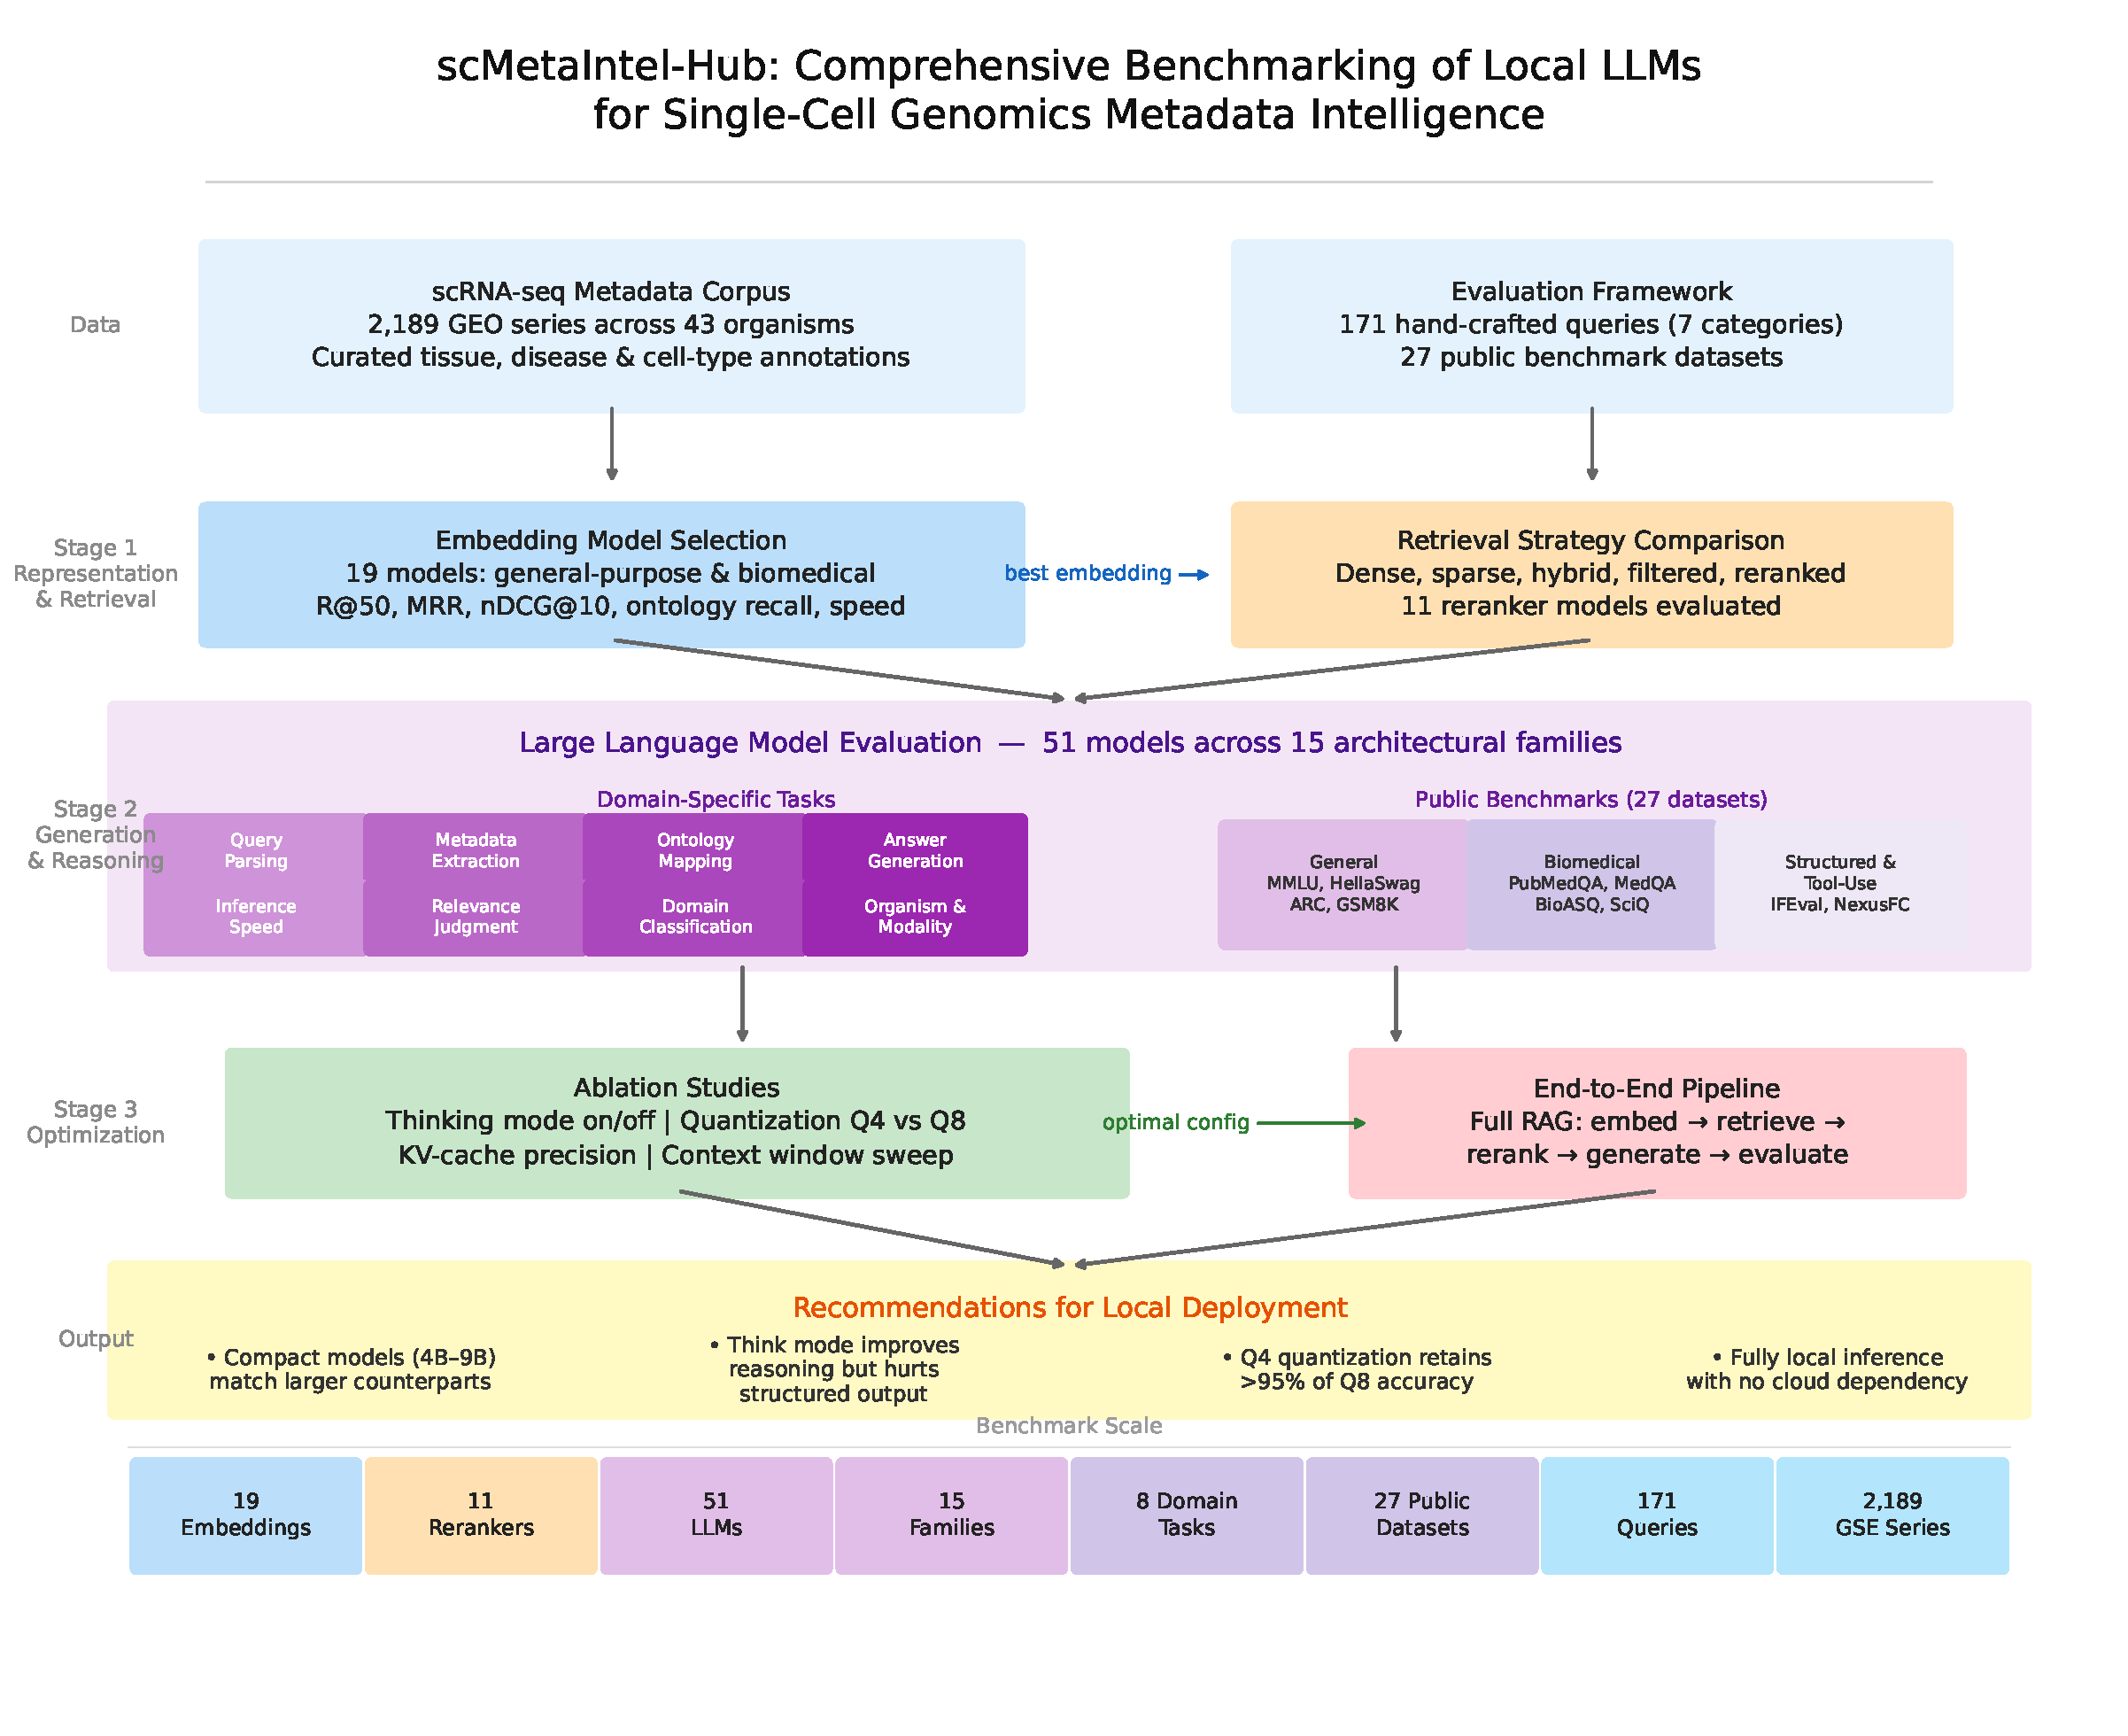
\includegraphics[width=\textwidth]{fig1_study_design}
\caption{\textbf{scMetaIntel-Hub pipeline overview.} The system processes
  natural-language queries through five stages: query parsing, document
  embedding, hybrid retrieval with organism filtering, context assembly,
  and cited answer generation. All components run locally on a single GPU.}
\label{fig:design}
\end{figure}

\begin{figure}[t]
\centering
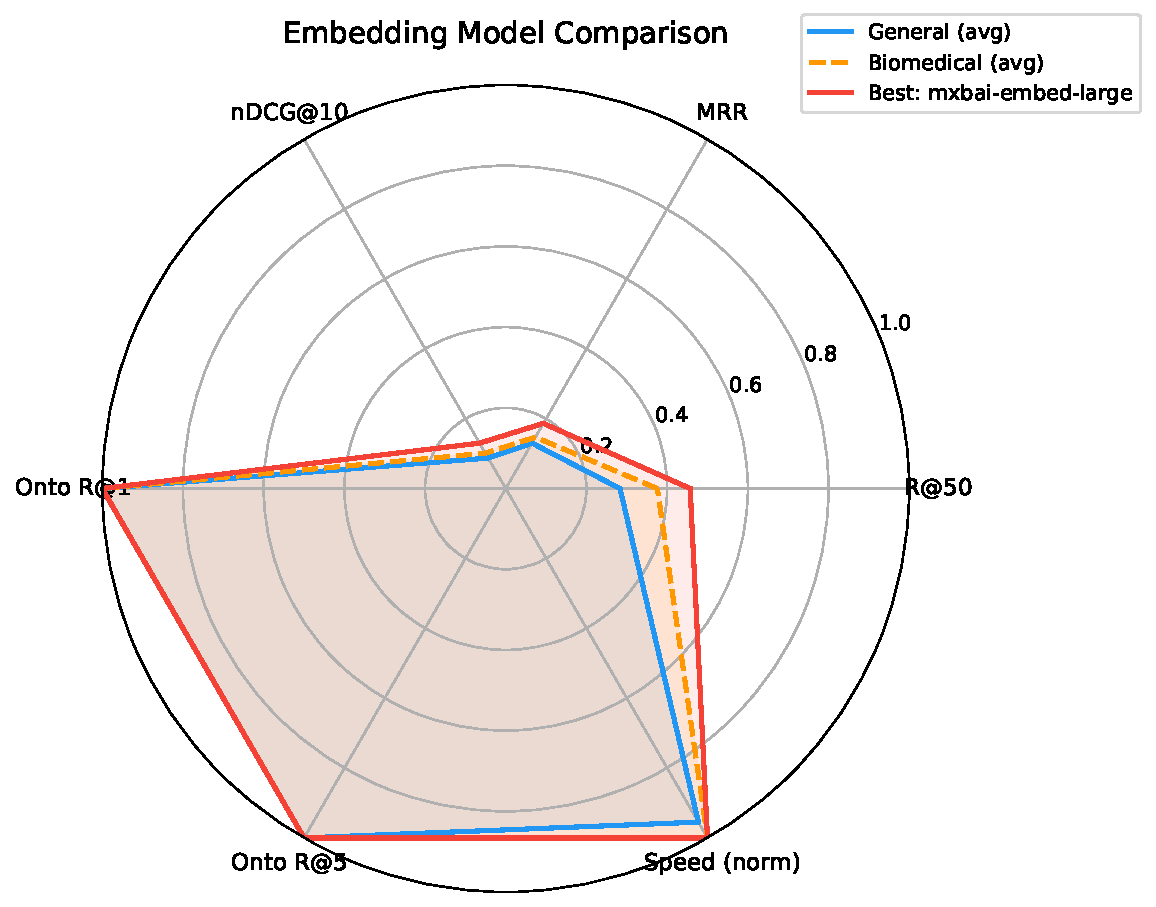
\includegraphics[width=\textwidth]{fig2_embedding_radar}
\caption{\textbf{Embedding model comparison.} Performance of 14 models
  (10 general-purpose, 4 biomedical) across retrieval recall, ontology
  matching, semantic clustering, and encoding speed. mxbai-embed-large
  achieves the highest retrieval R@50 (0.457) while biomedical models
  lead on ontology matching.}
\label{fig:embedding}
\end{figure}

\begin{figure}[t]
\centering
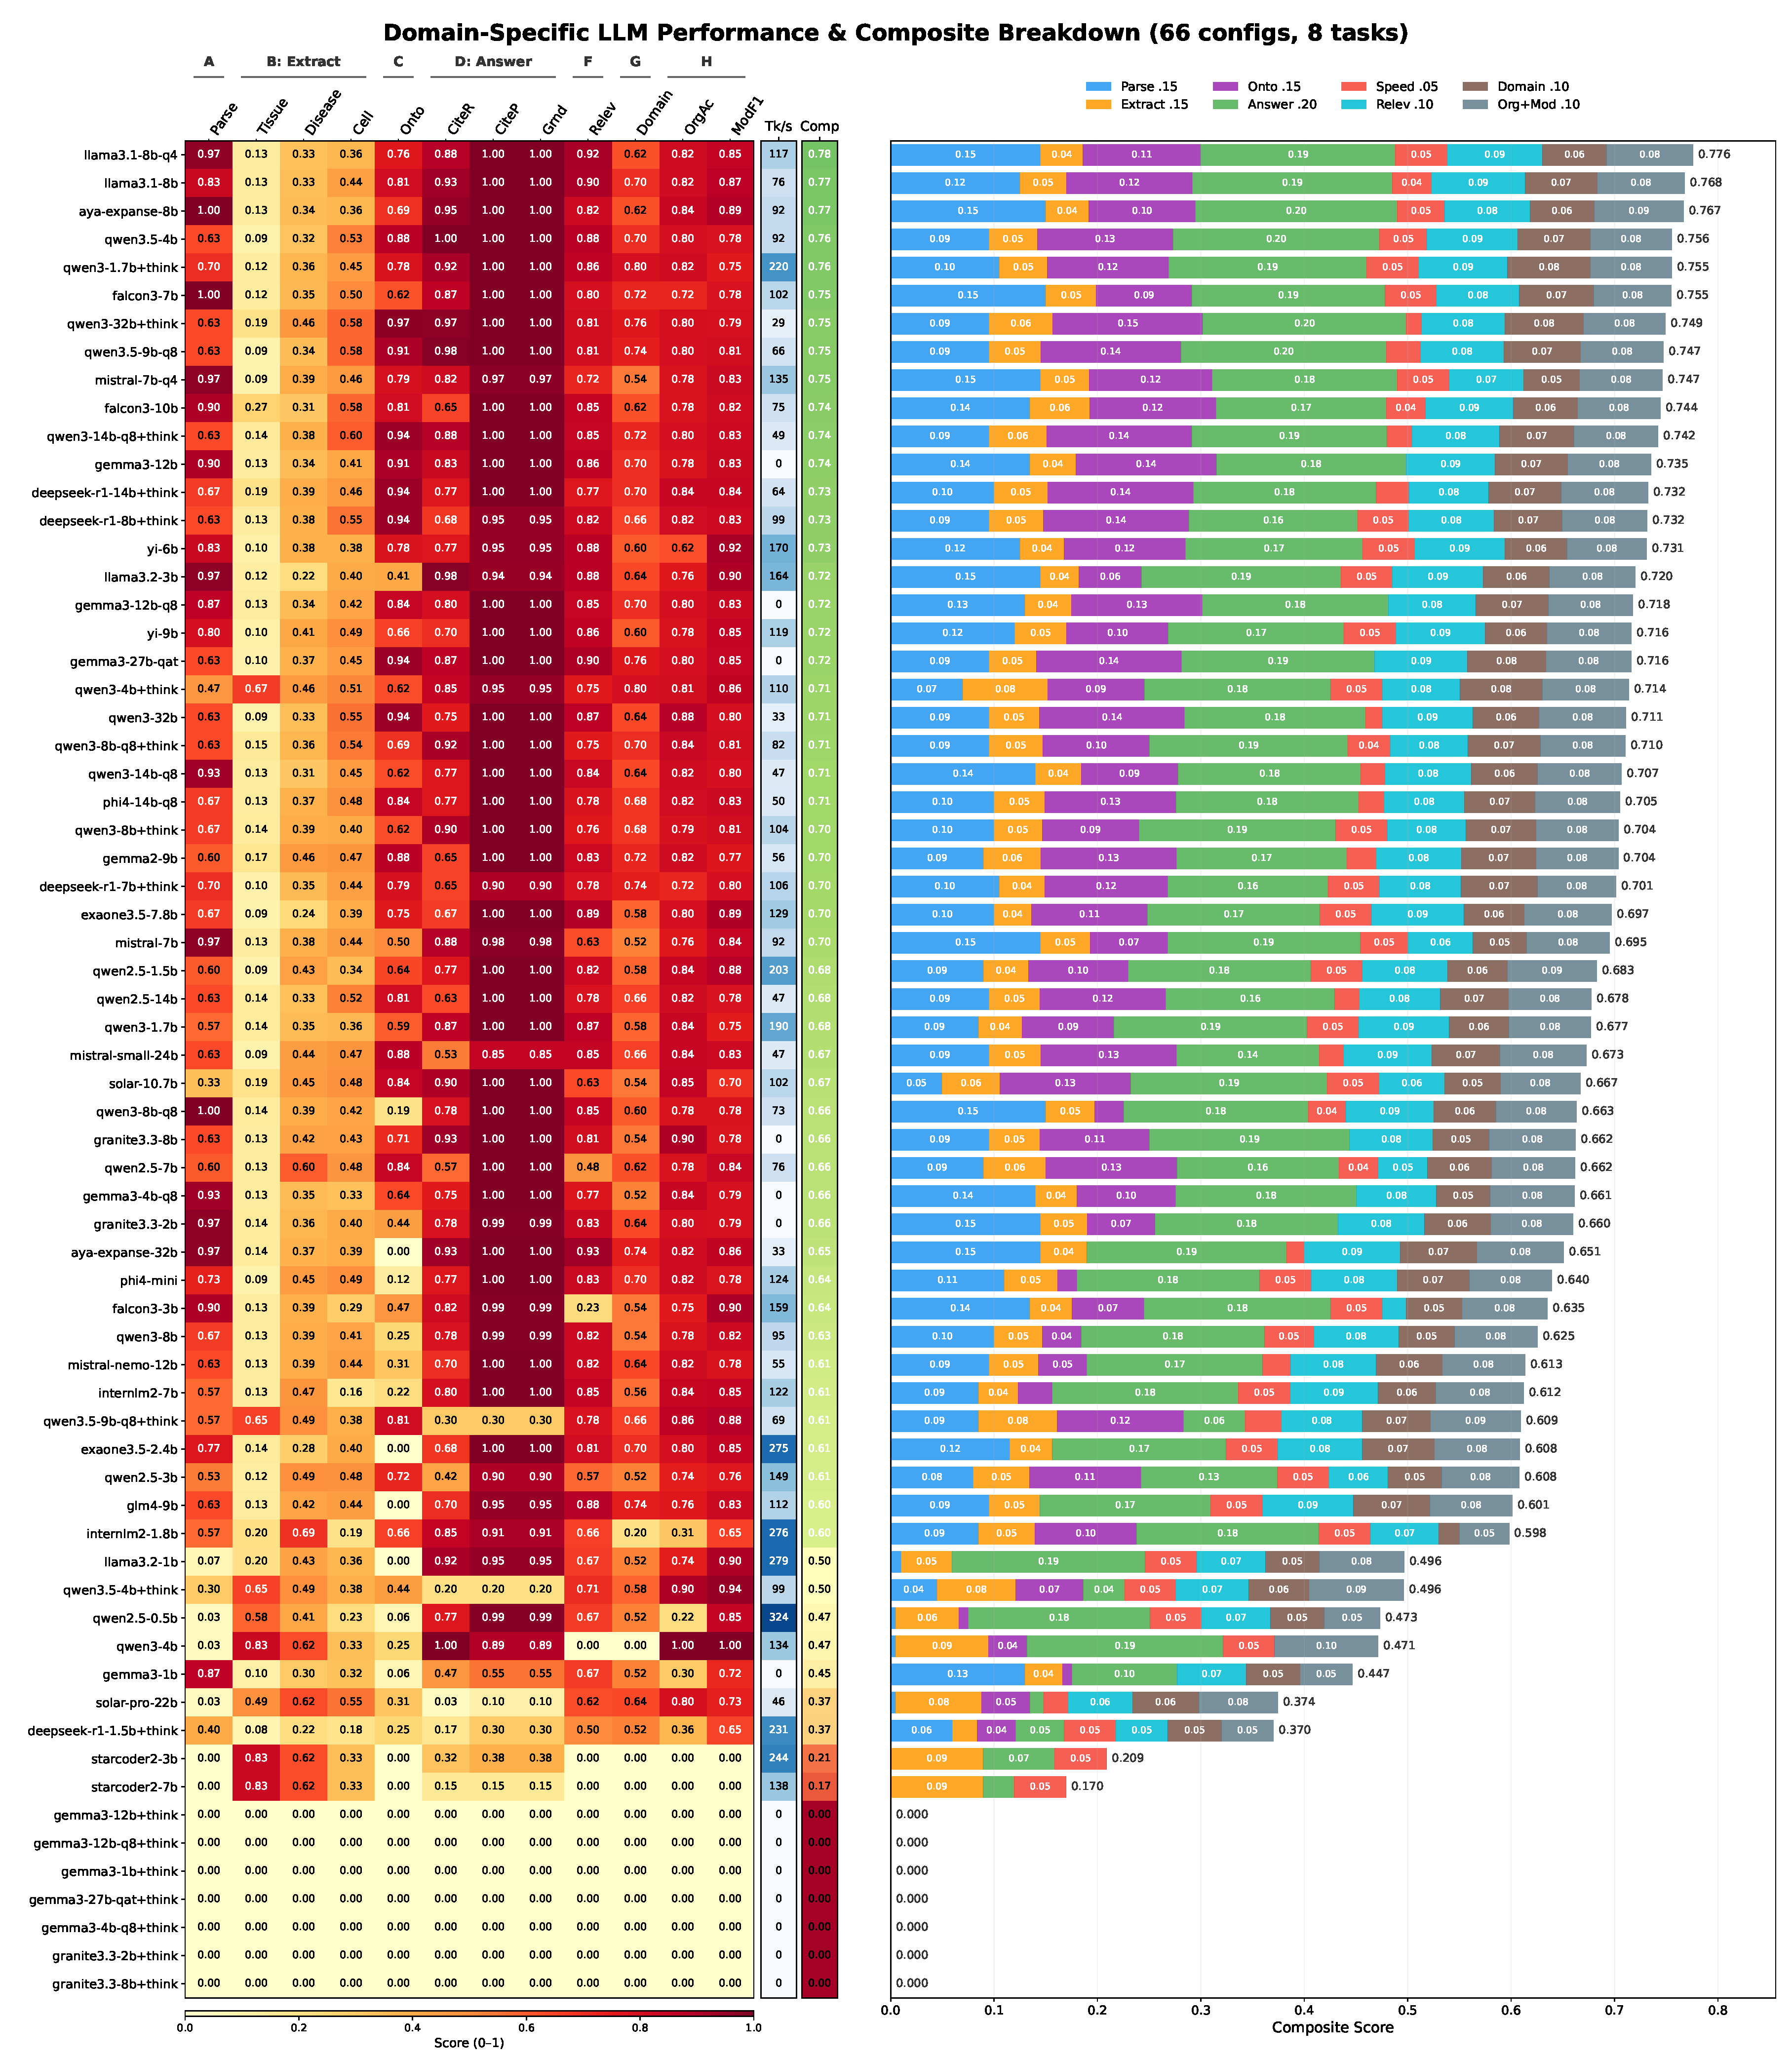
\includegraphics[width=\textwidth]{fig4_llm_heatmap}
\caption{\textbf{Per-task heatmap for all LLM configurations.} Rows are
  model configurations sorted by composite score; columns are the eight
  benchmark tasks. Colour intensity indicates normalised task score.
  Citation recall (Task~D) shows the widest variation and is the strongest
  predictor of overall rank.}
\label{fig:heatmap}
\end{figure}

\begin{figure}[t]
\centering
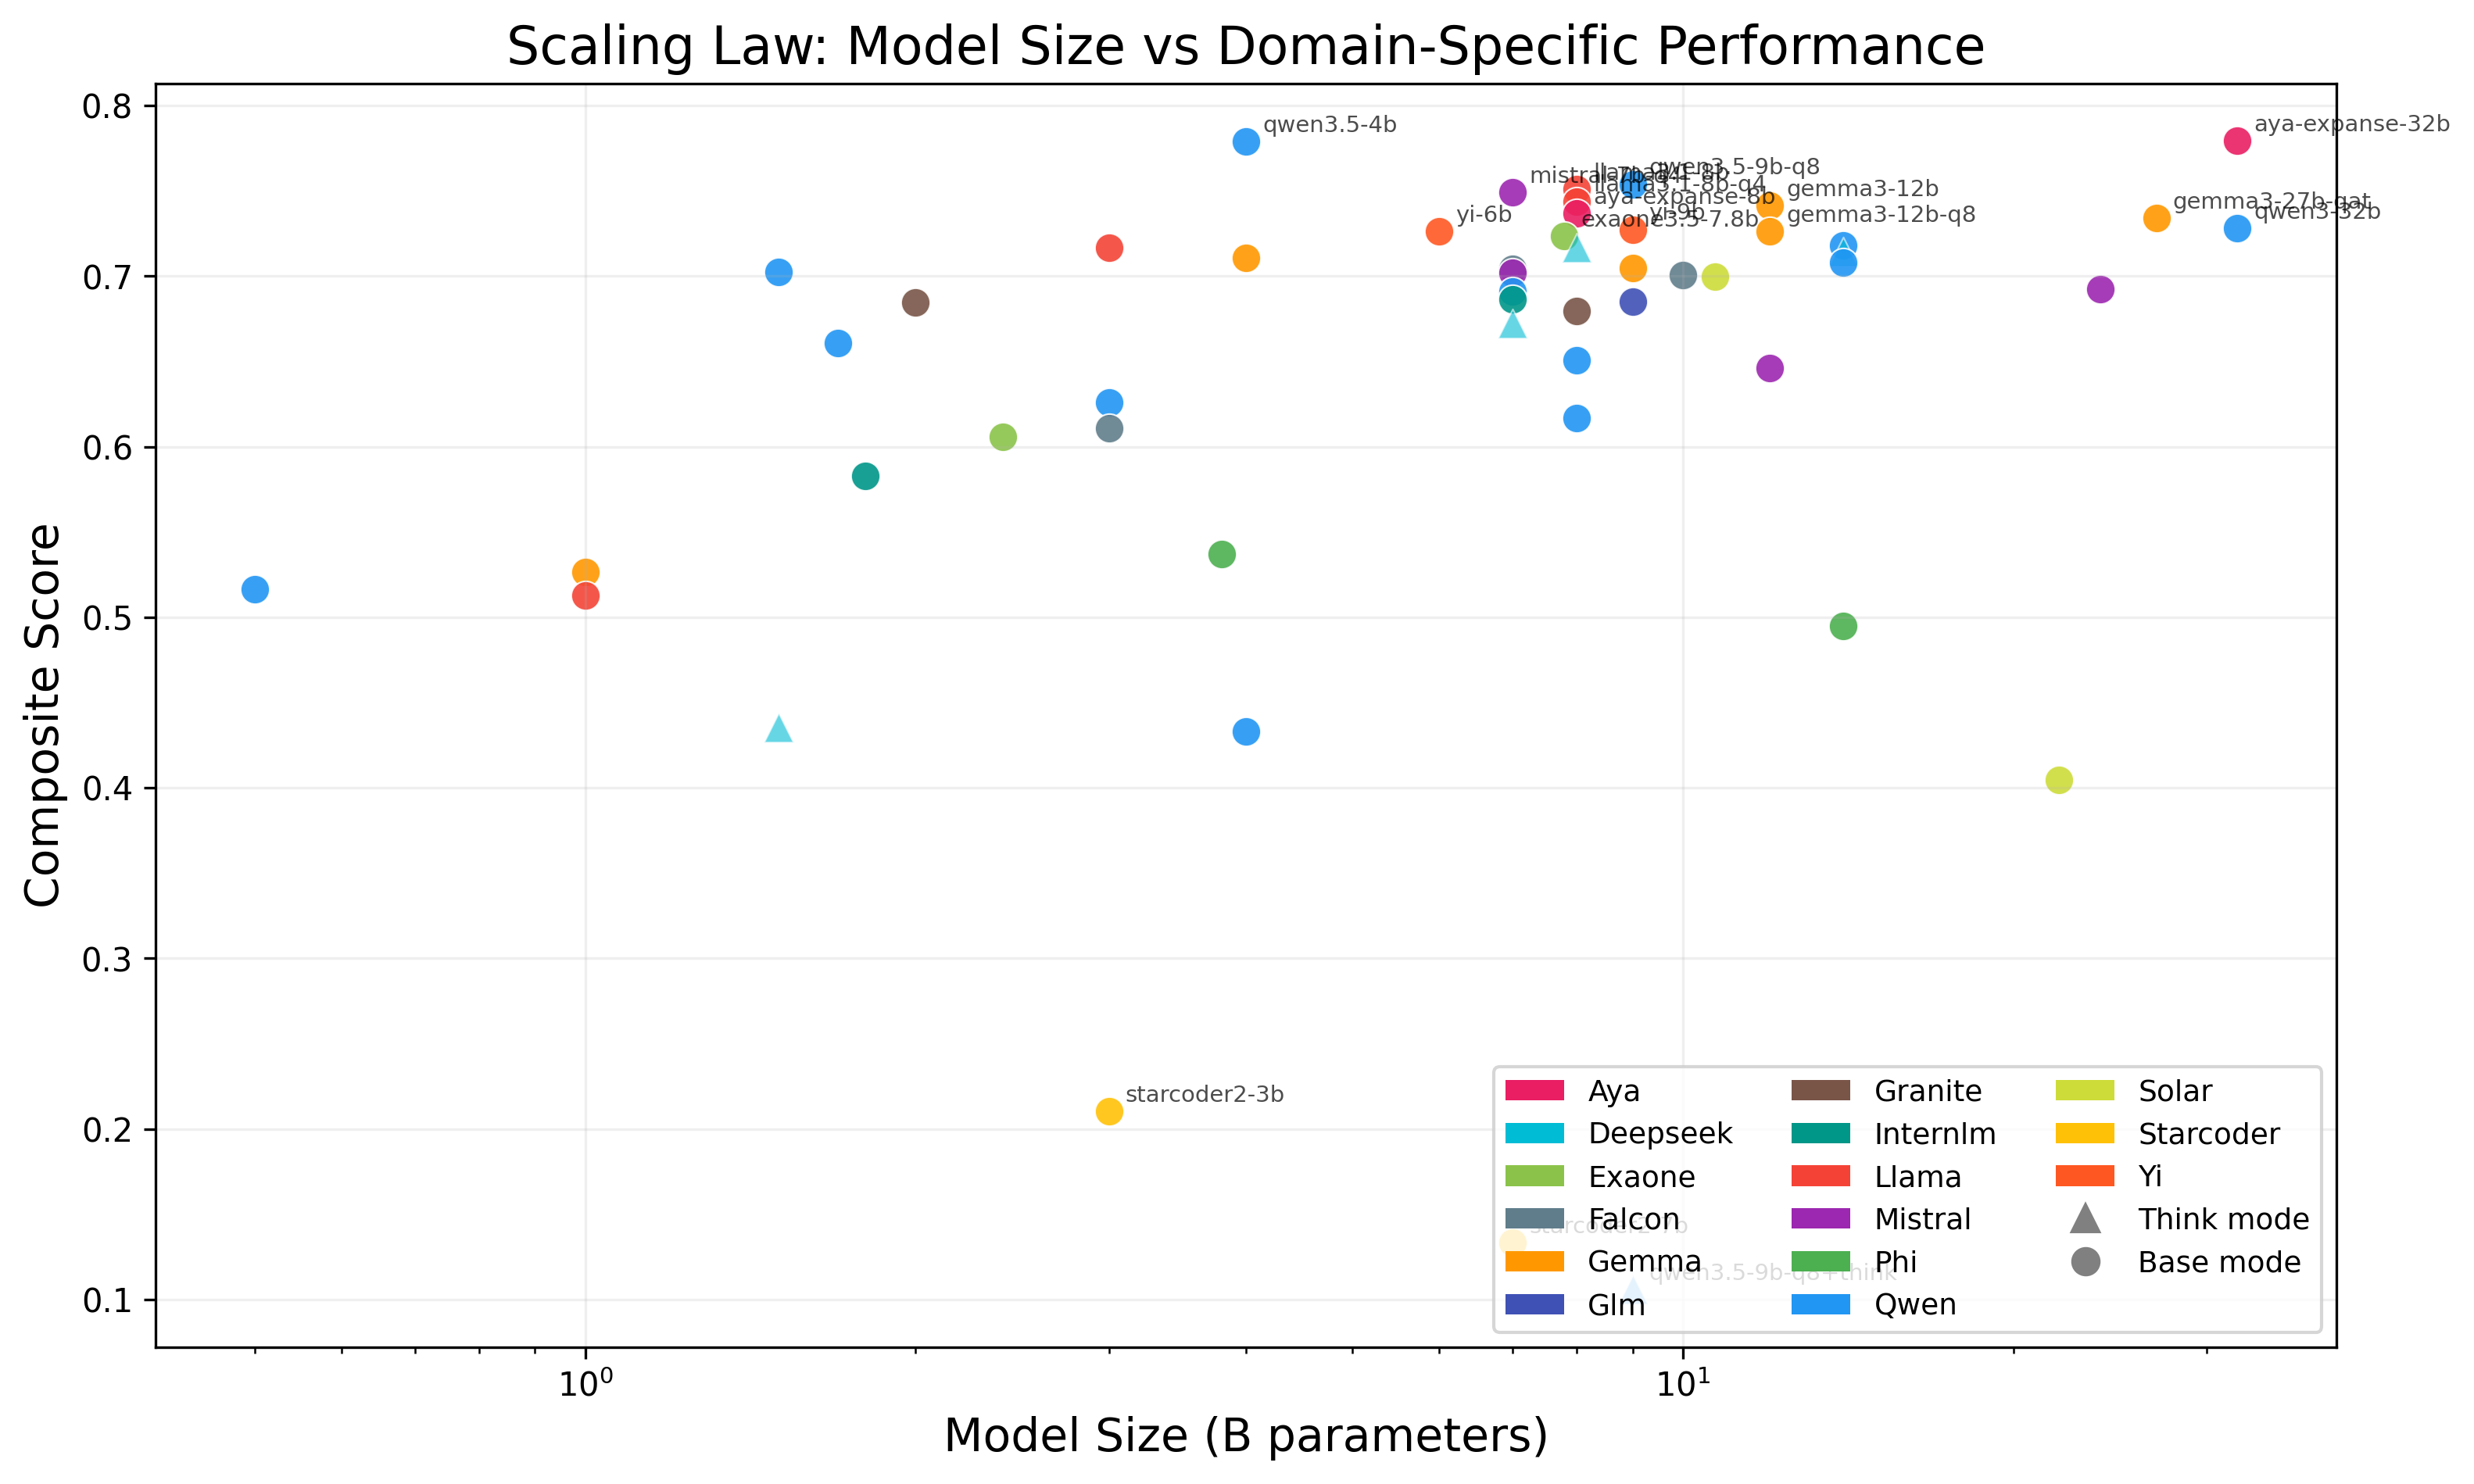
\includegraphics[width=0.7\textwidth]{fig_scaling_law}
\caption{\textbf{Composite score vs.\ model size.} Each point represents
  one configuration, coloured by model family. The weak negative Spearman
  correlation ($\rho = -0.08$) indicates that parameter count alone does
  not predict metadata-task performance.}
\label{fig:scaling}
\end{figure}

\begin{figure}[t]
\centering
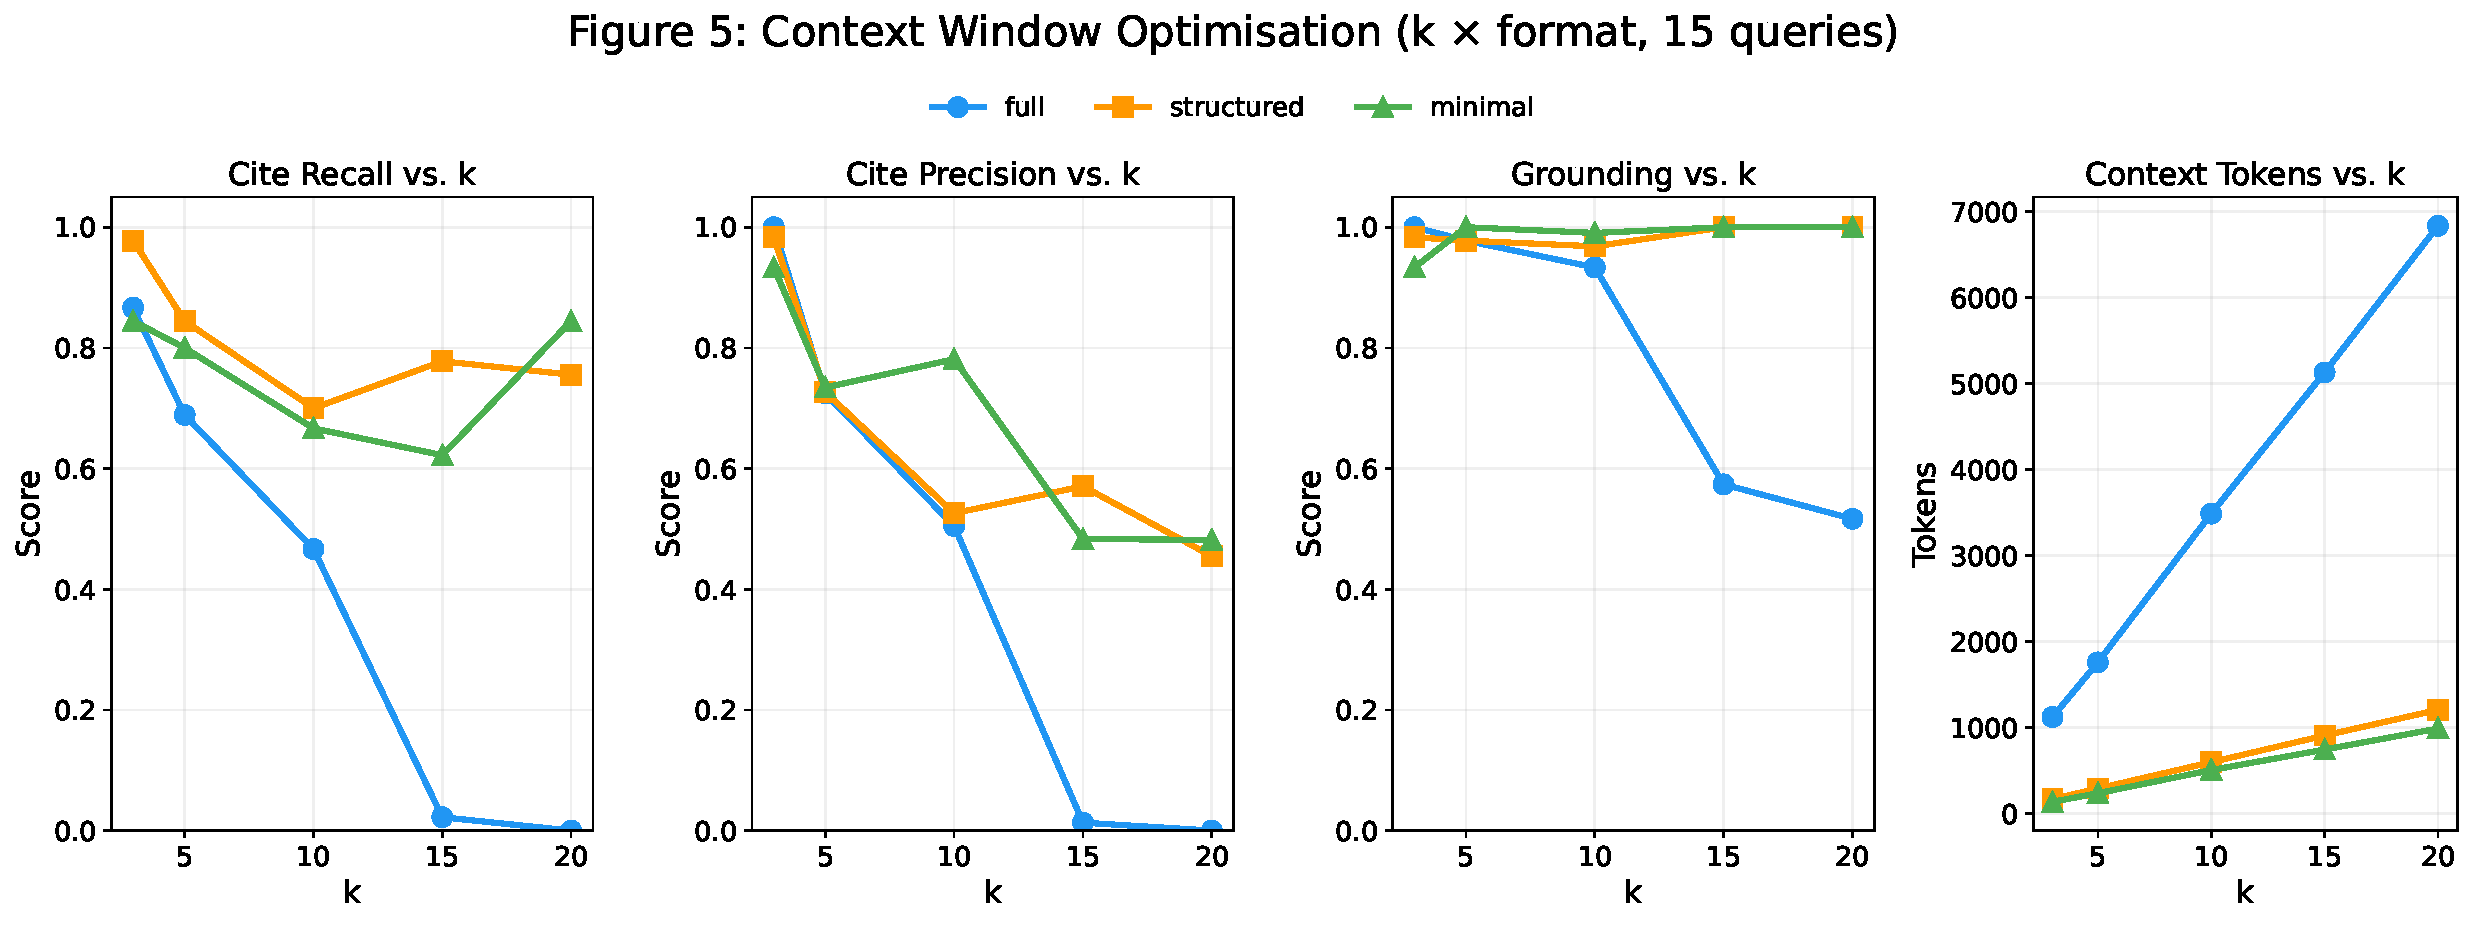
\includegraphics[width=\textwidth]{fig5_context_curve}
\caption{\textbf{Context window optimisation.} Citation precision,
  recall, and grounding rate as a function of format (full, structured,
  minimal) and top-$k$ (3, 5) across system-prompt variants. Structured
  format with $k = 3$ yields optimal performance.}
\label{fig:context}
\end{figure}

\begin{figure}[t]
\centering
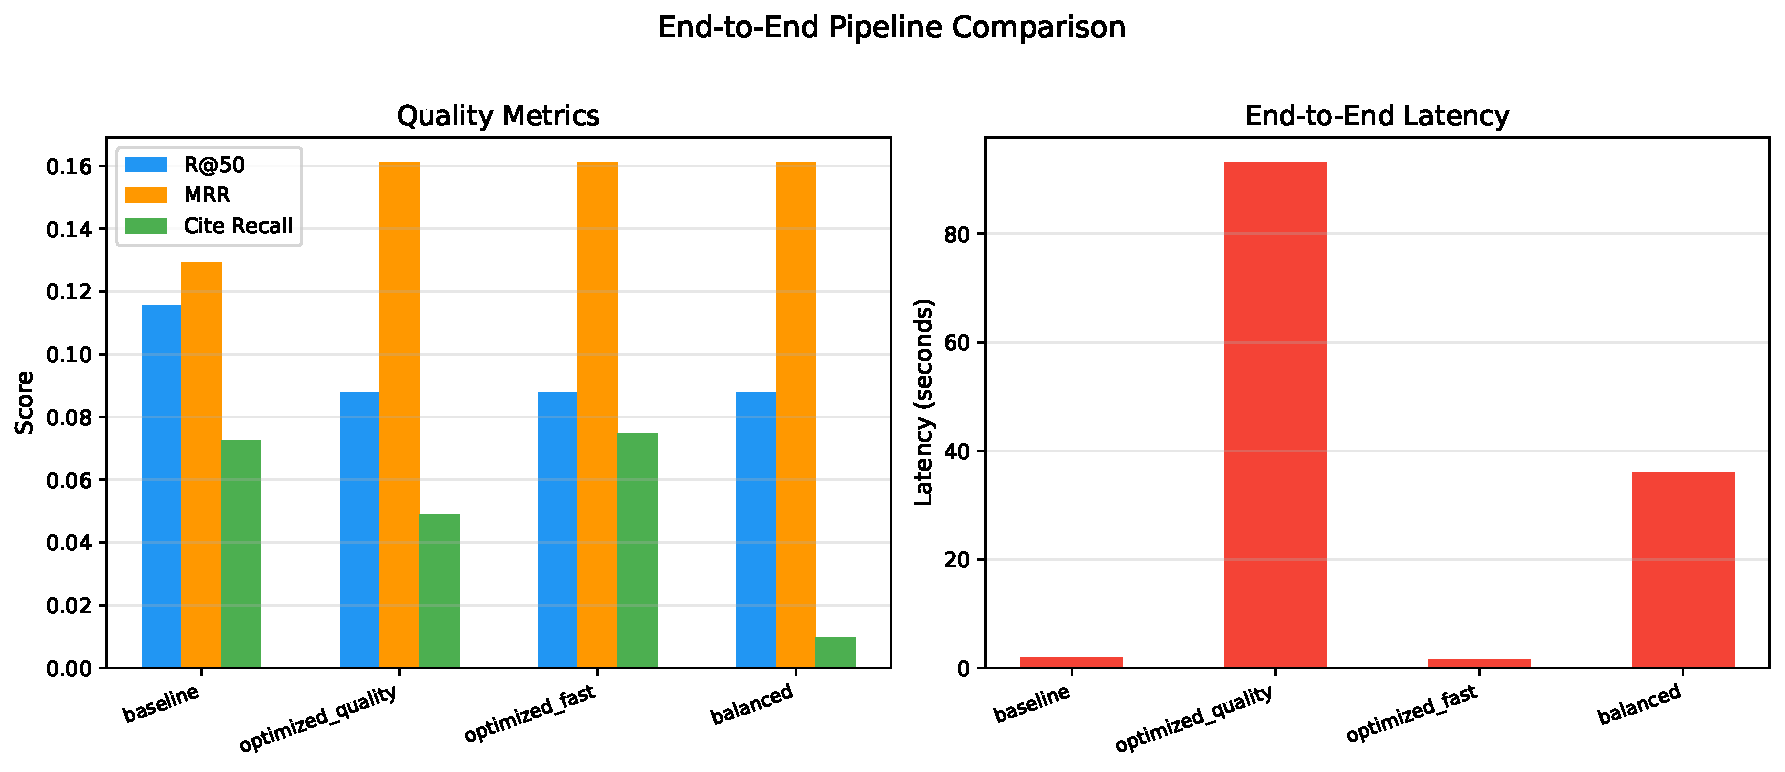
\includegraphics[width=\textwidth]{fig6_e2e_comparison}
\caption{\textbf{End-to-end pipeline comparison.} Four pipeline
  configurations (baseline, optimised-fast, balanced, quality-optimised)
  compared on citation recall, grounding rate, and latency. The
  optimised-fast pipeline achieves the best quality--latency trade-off.}
\label{fig:e2e}
\end{figure}

%% ====================================================================
%% References
%% ====================================================================
\bibliography{references}

\end{document}
